\section{Reward-Based Latent Hazard Model}

Rosenberg et al. (2021) propose computational methods to explain abrupt shifts in behavior in the maze experiment. One possibility is gradual reinforcement learning, where behavioral biases accumulate slowly through repeated reward feedback \cite{sutton2018}. Another possibility is that animals abruptly change their strategies after accumulating sufficient evidence for the optimal path. To explore these possibilities, they expand upon the original Rosenberg modeling framework by comparing three alternative models of learning dynamics: the gradual learning model, the latent hazard model, and the forced insight model.

The behavioral trajectory of a mouse in the maze is represented using a second-order Markov model defined on the maze graph. At each step, the next state depends on the current node, the previous node and a transition probability matrix. The model uses four behavioral bias parameters:
\begin{equation}
b_i = (B_f, B_a, L_f, L_o)
\end{equation}

Where $B_f$ is the probability of moving forward rather than returning to the parent node, $B_a$ is the probability of alternating direction after forward movement, $L_f$ is the probability of leaving a branch rather than backtracking and $L_o$ is the probability of exiting toward the outer maze. These parameters define the transition tensor:
\begin{equation}
T(s_{t-1}, s_t , s_{t+1})
\end{equation}

\subsection{Gradual Learning Model}
The incremental learning model updates behavioral bias using reward-dependent Bayesian updates. After the reward is received, the pseudo-numbers are updated as follows:
\begin{equation}
a_i = a_i + \eta \cdot N_i^{reward}
\end{equation}

\begin{equation}
 b_i = b_i + \eta 
\cdot N_i^{nonreward}
\end{equation}
where:
\begin{itemize}
    \item $a_i, b_i$ are Beta distribution parameters
    \item $\eta$ is the learning rate
    \item $N_i$ represents transition counts
\end{itemize}
Within the model, the Beta distribution restricts transition probabilities to between 0 and 1, providing a natural conjugate prior distribution for Bernoulli processes \cite{bishop2006}.

\subsection{Latent Hazard Insight} 
The Reward-Based Latent Hazard Model, instead of making incremental parameter updates, assumes that insight occurs when sufficient reward evidence accumulates and switches between two behavioral modes:
\begin{equation}
 b^{explore} = (0.778, 0.728, 0.827, 0.655) 
\end{equation}
The exploration parameters correspond to the baseline behavioural biases reported in Rosenberg et al. (2021).
\begin{equation}
b^{exploit} = (0.928, 0.728, 0.907, 0.655)
\end{equation}
The exploitation parameters increase forward and branch-following biases, reflecting more efficient reward-directed navigation after learning.
The probability of switching between these modes depends on the number of rewards observed:
\begin{equation}
p(\text{switch}) = \sigma \left(k (R - \theta)\right)
\label{eq:switch}
\end{equation}

\begin{figure}[htbp]
    \centering
    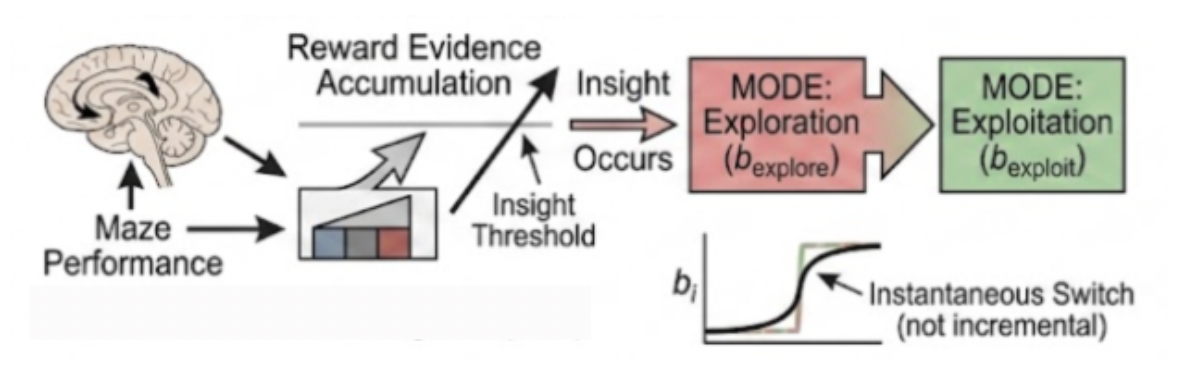
\includegraphics[width=\columnwidth]{figures/pbm_1.png}
    \caption{Schematic of the reward-based latent hazard mechanism: accumulated reward evidence increases the probability of an insight-triggered switch.}
    \label{fig:mechanism}
\end{figure}

To measure model performance, simulated trajectories were compared to the actual mouse trajectory using various goodness-of-fit metrics. 

\begin{figure}[htbp]
    \centering
    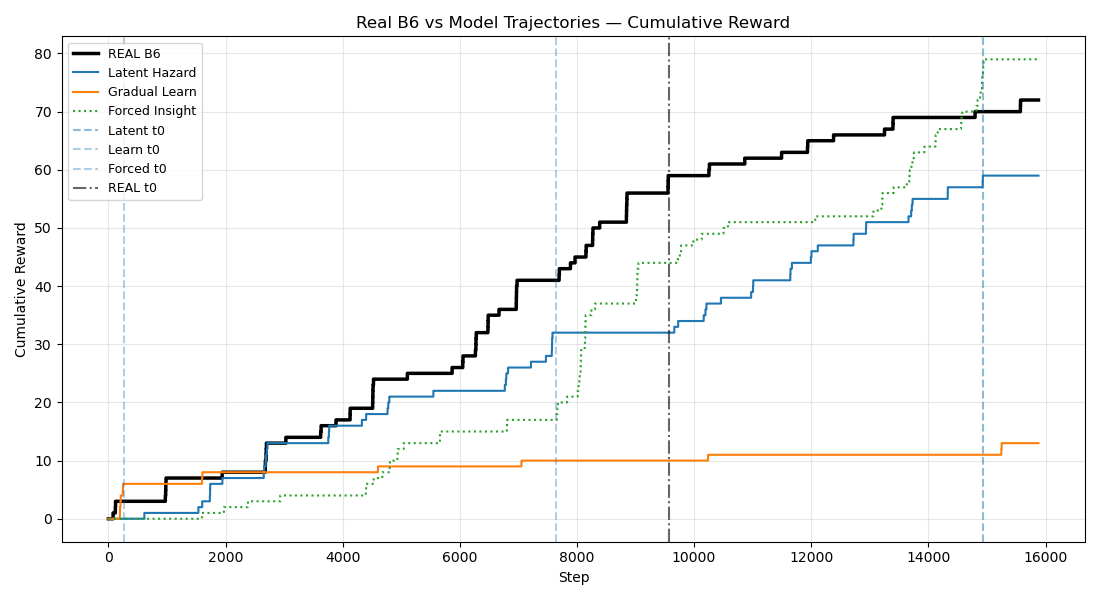
\includegraphics[width=\columnwidth]{figures/pbm_Figure_1.png}
    \caption{Model comparison of cumulative reward trajectories. The graph shows the cumulative reward trajectory of the B6 mouse used in the experiment compared with three simulation models: the Latent Hazard model, the Stepwise Learning model, and the Forced Insight model. The simulations were run with the same trajectory length (15,881 steps) to provide comparable goodness-of-fit assessments. Vertical dashed lines indicate the estimated point of change $(t_0)$ identified using reward rate change point analysis. While the latent hazard model reproduces a reward rate transition similar to the empirical trajectory, the stepwise learning model appears to fail to capture the abrupt behavioral change. The Forced Insight model produces a sharp transition but deviates from the true trajectory in overall reward accumulation.}
    \label{fig:trajectories}
\end{figure}

\begin{table}[htbp]
\centering
\caption{Quantitative Model Fit (Real B6 vs models; $n = 10$ seeds)}
\label{tab:model_fit}
\resizebox{\columnwidth}{!}{%
\begin{tabular}{lcccc}
\hline
Model & $\Delta t_0$ (med [Q1,Q3]) & MSE (mean $\pm$ SD) & $\Delta R_{tot}$ \\
\hline
Latent Hazard & 6134 [4293, 9028] & 130.94 $\pm$ 84.26 & 16.8 $\pm$ 9.4 \\
Gradual Learn & 8704 [8021, 9188] & 1494.56 $\pm$ 162.91 & 58.1 $\pm$ 3.1 \\
Forced Insight & 8247 [4574, 8973] & 71.30 $\pm$ 43.80 & 8.1 $\pm$ 6.9 \\
\hline
\end{tabular}%
}
\end{table}
As shown in Figure 1 and quantified in Table 1, the gradual learning model shows substantially larger trajectory error (MSE), whereas the latent hazard model provides a better overall balance between change-point timing and cumulative trajectory fit.

\subsection{Model Calibration}

To identify biologically plausible parameters for the latent hazard model, 
a grid search was performed over the switching threshold ($\theta$) and 
hazard sharpness parameter ($k$). Candidate parameter values were

\begin{equation}
\theta \in \{6,8,10,12,14\}, \quad
k \in \{0.2,0.4,0.6,0.8\}
\end{equation}

For each parameter pair, simulations were repeated across multiple random 
seeds ($n = 10$). The resulting trajectories were compared with the real 
B6 mouse trajectory using several goodness-of-fit metrics.

To select the best parameter combination, a composite score was constructed 
by normalizing and combining the following metrics:

\begin{itemize}
\item change-point timing error ($\Delta t_0$)
\item reward difference at the transition ($\Delta Reward_{t0}$)
\item cumulative trajectory error (MSE)
\item transition width difference ($\Delta w$)
\item slope ratio difference ($|\Delta \log SR|$)
\end{itemize}

The parameter pair minimizing the composite score was selected as the 
optimal latent hazard configuration.
\subsection{Change-Point Detection}

To estimate the timing of the behavioral transition, we applied a 
change-point detection procedure to the cumulative reward trajectory. 
The reward increment series was smoothed and approximated by a 
two-segment piecewise model representing pre- and post-insight reward rates.

The optimal transition point $t_0$ was defined as the point that minimizes 
the sum of squared errors (SSE) across the two segments:

\begin{equation}
t_0 = \arg\min_{t} (SSE_{pre}(t) + SSE_{post}(t))
\end{equation}

where $SSE_{pre}$ and $SSE_{post}$ represent the squared deviations of the 
reward increments from the estimated reward rate before and after the 
transition point.
\subsection{Transition Width}

To quantify the abruptness of the behavioral transition, we measured the 
transition width ($w$), defined as the interval between the 10\% and 90\% 
increase in the smoothed reward acquisition rate:

\begin{equation}
w = t_{90\%} - t_{10\%}
\end{equation}

Following Rosenberg et al. \cite{rosenberg2021}, transitions with $w < 300$ steps are interpreted as evidence for sudden insight rather than gradual learning.
\subsection{Slope Ratio Metric}

To quantify the increase in reward collection efficiency after insight, 
we computed the slope ratio (SR), defined as the ratio between post-transition 
and pre-transition reward acquisition rates:

\begin{equation}
SR = \frac{r_{post}}{r_{pre}}
\end{equation}

where $r_{pre}$ and $r_{post}$ represent the average reward rates before 
and after the estimated change-point.

For model comparison we evaluated the absolute difference between the 
logarithmic slope ratios of simulated and real trajectories:

\begin{equation}
|\Delta \log SR|
\end{equation}

which captures discrepancies in the magnitude of reward-rate acceleration.